\chapter{CHM compiler}

Our implementation of the CHM compiler uses preprocessing and postprocessing by gcc with the intermediate representation being the C language.

This allows us to focus on type inference and type checking instead of dealing with the meaning of the code, but the nature of this decision requires implementing some mangling of names to give instances unique names.

\section{Language extensions}

The C language is extended with polytyped functions and structures for parametric polymorphism and by an addition of type classes which offer a way of controlled ad-hoc polymorphism.

These extensions are explained more closely in the previous chapters in the context of the type system, here we will describe an actual application of them.

We will borrow the application from the haskell language, however in haskell there is a clear distinction between variables and non-variables. In C we don't have this distinction grounded in the core of the language and we want to preserve it as much as possible.

So to preserve the syntactic principles of the C language we will use a syntax similar to languages like C++, Java, C\#, etc. Those languages have become very popular and so it shouldn't be a bad choice. % FIXME: pls reword this, and upwards

\subsection{Polytyped Definitions}

We will explain polytyped (generic) definition on this example of a definiton of a class:

\begin{lstlisting}
    <a>
    class PseudoPointer
    {
        void deref(a);
    }
\end{lstlisting}

Here we see the part \lstinline{<a>}, similar to C++'s templates and to Java generics, but in this syntax always preceding the rest of the definition. This part has the following grammar rule: % TODO: give it a name

$:= <type\_declarations> | <type\_declarations : constraints> | < : constraints >$

Where the \emph{type\_declarations} is a list of new type variables and \emph{constraints} is a list of predicates and new type definitions (which are very similar to typedefs).

\subsubsection{Type Classes, Their Instances and Structs}

The previous example shows how we would define a simple \emph{type class}, here we declare only one type we use in declarations of the class's methods and so it is implicitly considered it's type parameter. The type parameter can be specified explicitly following the name of the class:

\begin{lstlisting}
    <a>
    class PseudoPointer<a>
    {
        void deref(a);
    }
\end{lstlisting}

We will then use similar syntax for application of types to its \emph{instances} (and in other contexts where we apply types to something).

For \emph{structs} we will use a very similar syntax to the first example of a type class definition.

\subsubsection{Functions}

Functions will use the very same syntax, however with a slightly different behavior, they don't have any type parameters and instead they have type schemes such that their qualified types (containing the predicates specified following the type declarations) are quantified over the declared types.

\section{Parsing}

Parsing of the code is handled by the language-c project, originally meant for c99, which is slightly modified into language-chm. % TODO: visq/language-c

This project is used for output of pretty-printed C code as well.

\section{Type inference}

For the type inference we use the thih project, % TODO: thih
but using it sensibly requires some modifications to be made, then there are some more modifications as the original thih project isn't meant to be a real implementation.

Using thih requires a significant pre/post-processing of the code, described in the previous chapter. % TODO: modelling

The main parts of preprocessing the code are in the AST-to-THIH project, postprocessing is then in the CHM-instantiate project which also passes parts of the code to AST-to-THIH. Both of these projects are specifically built for this thesis.

All type inference principles are explained in the first chapter. The basis for the implementation is then explained in % TODO: thih

\section{Monomorphization and Instantiation} % TODO: fix name

Monomorphization of functions begins with monotype functions and then continues recursively when we determine the monotypes of all occurrences of polytype functions called from them.

Similarly for types (and namely structs).

We will describe the process only on functions, but the principles of it carry to structures as well.

We start with monotype functions as we can already determine their monomorphic type. We replace all polymorphic symbols in their definitions with unique symbols (distinct even if the original symbol was the same) with each assigned a new unique type variable. We run the type inference algorithm on this rewritten definition and then if we successfully determined each monotype we instantiate each of the original symbols given the new inferred type (unless we have done so already - this implies we have to keep a record of all instances).

Instantiation of polytyped functions is done by simply replacing the quantified type variables with the types so its resulting type scheme matches the one inferred for its occurrence in the caller. From there the process repeats as if the instance was a regular monomorphic function, there is one exception to this being type class methods which we will discuss in the very next part.

\subsection{Type class preprocessing}

All type classes are just language constructs, they are not manifested in the resulting code in any shape or form and thus they count as a zero abstraction feature. There are some built-in type classes, % TODO: list the type classes
implicit type classes for each field of a structure (and a union) and then user-defined type classes before in this chapter.

Definitions of user-defined type classes are stored in the compiler as lists of their methods that act like regular polytypes until we instantiate them. All methods defined in type classes are replaced by functions with a single predicate constraint on the type parameter of the type class.

When a method is instantiated the compiler checks its instances and determines which one matches the type scheme of the intended instance. Then it instantiates this one method instance.

% FIXME: continue from here...

\subsection{Record fields}

Implementing record fields was challenging as the way record fields work in C has no real equivalent in the context of functional programming, although haskell's object notation or ML's records come pretty close to it.

Record fields are implemented in such a way that we require the fields to be named differently or to have the exact same type, all other situations are not specified as this cannot be statically expressed in HM type system in any sensible way.

\subsection{Recursion limits}

It is indeterminable whether instantiation of something continues forever. We can prove this using post correspondence problem % FIXME: prove it

So there is a limit of type depth set to 500 (this limit shouldn't affect any sensible program).
% FIXME: Changing this limit is possible by adding an option --type-depth=N to the compiler (it can be also used to make stricter constraint as well).
If some type exceeds this limit, an compilation error will be outputted stating what the compiler was instantiating at that time.

\subsection{Comparison to C++ template instantiation}

One could say this project just mirrors template instantiation from C++, but any such resemblance is just superficial, C++ template instantiation is not strict in type signatures and different instances can have
non-matching types.

One example of this would be:

% FIXME: continue from here

\begin{lstlisting}
template<typename>
struct function_type;

template<>
struct function_type<int> { using return_type = int; using parameter_type = int; };

template<>
struct function_type<int*> { using return_type = int; using parameter_type = int*; };

template<>
struct function_type<int**> { using return_type = int*; using parameter_type = int; };

template<typename T>
typename function_type<T>::return_type function(typename function_type<T>::parameter_type);

template<>
int function<int>(int value) { return value; }

template<>
int function<int*>(int *value) { return *value; }

template<>
int *function<int**>(int value) { return &value; }
\end{lstlisting}

C++ allows different instances to have the same type signature which can make any type inference or type deduction
impossible.

One more difference is that C++ allows function overloading. % TODO: write about the paper linked by mirek

The instantiation in CHM follows inferred types by the HM type system.

\section{Code output}

The CHM compiler outputs gcc-compilable code which interprets the CHM code without any runtime overhead. % TODO: or at least I hope so

There are options allowing the user to see the inner haskell representation of the CHM code (it blurs some of the semantics unnecessary for type inference and leaves others to facilitate the readability of it), this can be used for debugging the compiler implementations. % FIXME: list the options (unimplemented yet)

It should be noted that names of symbols of polytype functions actually used in the C interpretation of the CHM code do not match their CHM counterparts which currently complicates debugging of CHM programs (this however can be solved easily on the debugger side).

\iffalse
\chapter{Results and discussion}

Instead, try some of the following:
\begin{itemize}
\item State a hypothesis and prove it statistically
\item Show plots with measurements that you did to prove your results (e.g. speedup). Use either \texttt{R} and \texttt{ggplot}, or Python with \texttt{matplotlib} to generate the plots.\footnote{Honestly, the plots from \texttt{ggplot} look \underline{much} better.} Save them as PDF to avoid printing pixels (as in ).
\item Compare with other similar software/theses/authors/results, if possible
\item Show example source code (e.g. for demonstrating how easily your results can be used)
\item Include a `toy problem' for demonstrating the basic functionality of your approach and detail all important properties and results on that
\item Include clear pictures of `inputs' and `outputs' of all your algorithms, if applicable
\end{itemize}

\begin{figure}
\centering
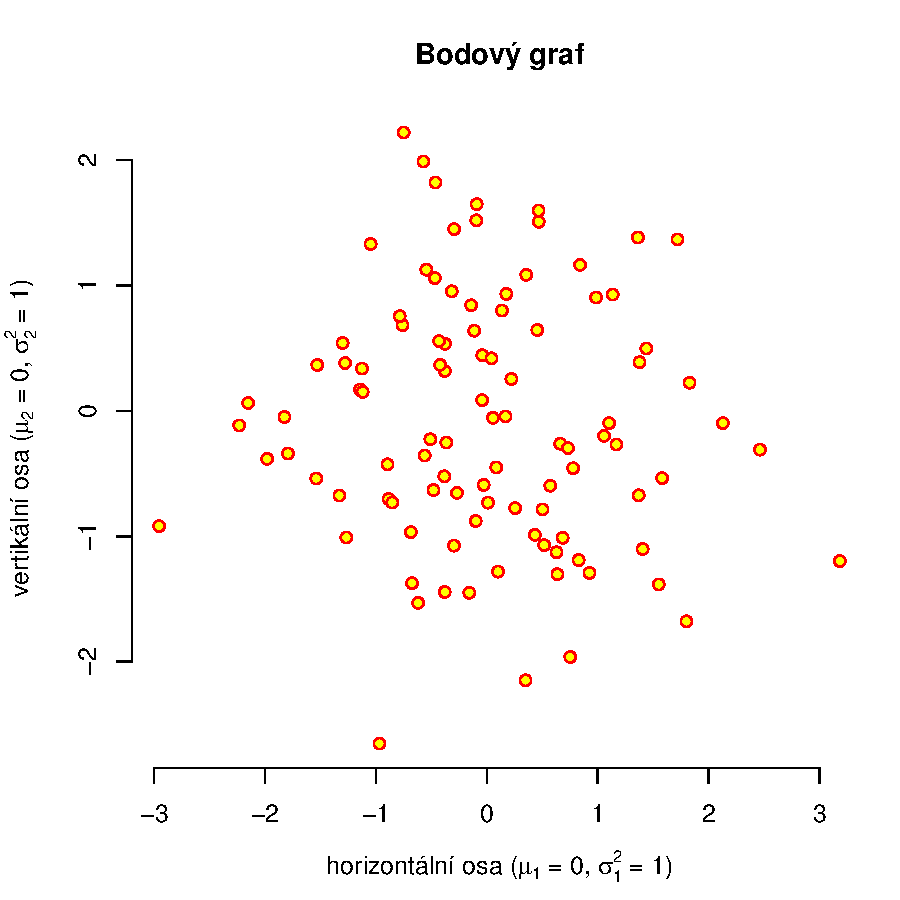
\includegraphics[width=.6\linewidth]{img/ukazka-obr01.pdf}
\caption{This caption is a friendly reminder to never insert figures ``in text,'' without a floating environment}
\label{fig:f}
\end{figure}

It is sometimes convenient (even recommended by some journals, including Cell) to name the results sub-sections so that they state what exactly has been achieved. Examples follow.

\section{SuperProgram is faster than OldAlgorithm}
\subsection{Scalability estimation}
\subsection{Precision of the results}
\section{Weird theorem is proven by induction}
\section{Amount of code reduced by CodeRedTool}
\subsection{Example}
\subsection{Performance on real codebases}
\section{NeuroticHelper improves neural network learning}

\section{What is a discussion?}
After you present the results and show that your contribution works, it is important to \emph{interpret} them, showing what they mean for the more general public.

Separate discussion sections are common in life sciences where ambiguity is common and intuition is sometimes the only thing that the authors have; exact sciences and mathematicians do not use them as often. Despite of that, it is nice to precisely set your output into the existing environment, answering:
\begin{itemize}
\item What is the potential application of the result?
\item Does the result solve a problem that other people encountered?
\item Did the results point to any new (surprising) facts?
\item Why is the result important for your future work (or work of anyone other)?
\item Can the results be used to replace (and improve) anything that is used currently?
\end{itemize}

If you do not know the answers, you may want to ask the supervisor. Also, do not worry if the discussion section is half-empty or completely pointless; you may remove it completely without much consequence. It is just a bachelor thesis, not a world-saving avenger thesis.
\fi
